% =============================================================================
% Module 11: Lensing Statistics and Cross-Sections
% =============================================================================
% Sources: Schneider, Kochanek & Wambsganss (2006), Part 1 (Schneider) Sec. 5;
%          Part 2 (Kochanek) Sec. 6. Narayan & Bartelmann (1997).
% Mathematica: ../Mathematica/11_Lensing_Statistics/
% =============================================================================

\chapter{Lensing Statistics and Cross-Sections}
\label{ch:lensing_statistics}

\begin{quote}
\textit{One is frequently interested in the probability that a specific
gravitational lensing event occurs.  The results of such an
investigation depend on the assumed distribution of lens masses and
their density profiles --- and a comparison with a well-defined sample
of observed lenses can constrain the lens population and the geometry of
the Universe.}
\hfill --- Schneider, Kochanek \& Wambsganss (2006), Part 1
\end{quote}

\noindent
So far we have studied lenses one at a time.  But a survey observes
\emph{populations}: many sources seen through many deflectors.  The
questions then become statistical --- what fraction of distant quasars is
multiply imaged?  how many giant arcs should a cluster survey find?  how
does lensing distort the number counts of a flux-limited sample?  These
questions are answered with three ingredients built in this module:
\begin{itemize}[nosep]
    \item the \textbf{cross-section} of a single lens for a given imaging
          property (\S\ref{sec:cross_sections});
    \item the \textbf{optical depth}, obtained by summing cross-sections
          over the lens population along the line of sight
          (\S\ref{sec:optical_depth});
    \item the \textbf{magnification bias}, which reshapes the observed
          counts of a lensed source population
          (\S\ref{sec:magnification_bias}).
\end{itemize}
Together these make lens statistics a probe both of the lens population
(masses, profiles, abundance) and of cosmology (through the volume
element).  We build on the point-mass and SIS imaging of
Modules~\ref{ch:lens_equation} and~\ref{ch:axisymmetric_models} and the
caustic structure of Module~\ref{ch:elliptical_models}.

\medskip
\noindent
\textbf{Companion Mathematica files:}
\begin{itemize}[nosep]
    \item \mathlink{11_Lensing_Statistics/lensing_statistics.wl}{lensing\_statistics.wl}
          --- symbolic derivation and verification of the point-mass and
          SIS cross-sections, the optical-depth integrand, and the
          magnification-bias factor for power-law counts; figures
          exported to \texttt{Figures/11\_Lensing\_Statistics/}.
\end{itemize}


% =====================================================================
\section{Lensing Cross-Sections}
\label{sec:cross_sections}

Fix a source and a lens at given distances.  For some imaging property
$Q$ --- ``total magnification exceeds $\mu$'', ``image separation exceeds
$\Delta\theta$'', ``flux ratio below $r$'' --- there is a region of the
\emph{source plane} in which the source must lie for the images to have
property $Q$.  The solid angle of that region is the \textbf{cross-section}
$\sigma_Q$
\citep[][Part~1, \S5.1]{schneider_kochanek_wambsganss_2006}.  Everything
in lens statistics is built from cross-sections.

\subsection{The Point-Mass Lens}
\label{sec:cross_point}

For a point mass there is a one-to-one relation between the scaled source
position $y = \beta/\thetaE$ and the total magnification
$\mu_p(y) = (y^2+2)/\big(y\sqrt{y^2+4}\big)$
(Module~\ref{ch:lens_equation}).  Inverting it, the source produces a
total magnification greater than $\mu_p$ whenever it lies within
\begin{equation}
    y^2(\mu_p)
    = 2\left(\frac{\mu_p}{\sqrt{\mu_p^2-1}} - 1\right),
    \label{eq:point_ymu}
\end{equation}
so the cross-section for magnification $>\mu_p$ is
\begin{equation}
    \sigma(\mu_p) = \pi\,\thetaE^2\,y^2(\mu_p).
    \label{eq:point_cross_mu}
\end{equation}
At high magnification $y^2 \to 1/\mu_p^2$, giving the universal
$\sigma \propto \mu_p^{-2}$ (equivalently the differential
$p(\mu)\,d\mu \propto -\,\tfrac{d\sigma}{d\mu}\,d\mu \propto \mu^{-3}\,d\mu$
that recurs in \S\ref{sec:magnification_bias}).  Similarly, the cross-section for the
image brightness ratio to be smaller than $r > 1$ is
\begin{equation}
    \sigma(r) = \pi\,\thetaE^2\left(r^{1/2} + r^{-1/2} - 2\right),
    \label{eq:point_cross_r}
\end{equation}
both verified symbolically in the companion script.

\begin{figure}[ht]
    \centering
    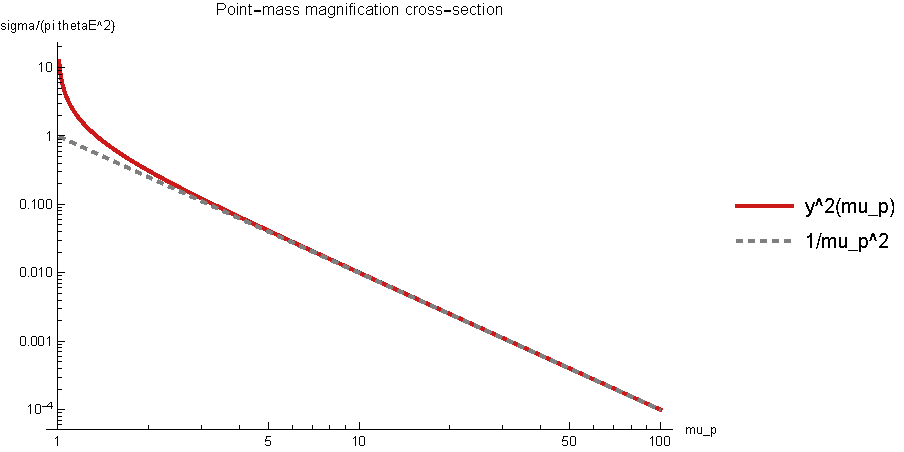
\includegraphics[width=0.72\textwidth]{../Figures/11_Lensing_Statistics/point_mass_cross_section.pdf}
    \caption{The point-mass magnification cross-section
    $\sigma(\mu_p)/(\pi\thetaE^2) = y^2(\mu_p)$ of
    Eq.~\eqref{eq:point_ymu}, as a function of the magnification
    threshold $\mu_p$.  At high magnification the cross-section falls as
    $\sigma \propto \mu_p^{-2}$ (dashed), the universal scaling that
    produces $p(\mu)\propto\mu^{-3}$ and drives the magnification bias.
    Generated by \texttt{lensing\_statistics.wl}.}
    \label{fig:point_cross}
\end{figure}

\subsection{The Singular Isothermal Sphere}
\label{sec:cross_sis}

The SIS (Module~\ref{ch:axisymmetric_models}) produces two images when
$\beta < \thetaE$, always separated by $2\thetaE$.  With
$y = \beta/\thetaE$, the total magnification and flux ratio of the pair
are
\begin{equation}
    \mu = \frac{2}{y}, \qquad r = \frac{1+y}{1-y}.
    \label{eq:sis_mu_r}
\end{equation}
The basic multiple-imaging cross-section is therefore simply the area of
the disk $\beta < \thetaE$,
\begin{equation}
    \sigma = \pi\,\thetaE^2,
    \label{eq:sis_cross}
\end{equation}
and with the resolution, magnification, and flux-ratio thresholds folded
in \citep[][Part~1, eq.~101]{schneider_kochanek_wambsganss_2006},
\begin{equation}
    \sigma(\Delta\theta, r, \mu)
    = \pi\,\thetaE^2
      \left[\min\!\left(\frac{r-1}{r+1},\,\frac{2}{\mu}\right)\right]^2
      H(2\thetaE - \Delta\theta)\,H(\mu - 2).
    \label{eq:sis_cross_full}
\end{equation}
Because the SIS Einstein radius scales as
$\thetaE \propto \sigma_v^2$ (Module~\ref{ch:galaxy_lensing}), the
multiple-imaging cross-section scales as
$\sigma \propto \thetaE^2 \propto \sigma_v^4$ --- the origin of the strong
sensitivity of lens statistics to the most massive galaxies.


% =====================================================================
\section{Optical Depth}
\label{sec:optical_depth}

The probability that a random source is lensed with property $Q$ --- the
\textbf{optical depth} $\tau$ --- is the fraction of the sky covered by
the cross-sections of all intervening lenses.  Summing the (non-overlapping)
cross-sections of lenses with proper number density $n$ along the line of
sight,
\begin{equation}
    \tau(Q) = \int_0^{z_s}\! dz_d\;
        D_{\mathrm{ang}}^2(z_d)\,\frac{dr_{\mathrm{prop}}}{dz}
        \int d\chi\; n(z_d,\chi)\,\sigma(Q; z_d, z_s, \chi),
    \label{eq:optical_depth}
\end{equation}
where $\chi$ collects the lens parameters (mass, velocity dispersion,
ellipticity)
\citep[][Part~1, \S5.2]{schneider_kochanek_wambsganss_2006}.  Written with
the comoving number density $n = (1+z)^3 n_{\mathrm{com}}$ and comoving
angular diameter distance $f_K$, this becomes the particularly clean
\begin{equation}
    \tau(Q) = \int_0^{w_s}\! dw\; f_K^2(w)
        \int d\chi\; n_{\mathrm{com}}(w,\chi)\,\sigma(Q; w, w_s, \chi).
    \label{eq:optical_depth_comoving}
\end{equation}
For a population of SIS galaxies with cross-section
$\sigma = \pi\thetaE^2 \propto \sigma_v^4$, integrating over the observed
velocity-dispersion function yields the classic result that the
multiple-imaging optical depth scales as
$\tau \propto n_{\mathrm{com}}\,(\sigma_v/c)^4$ times a cosmological
volume factor (Turner, Ostriker \& Gott 1984).  It is that volume factor
--- larger in a universe with a cosmological constant --- that once made
lens counts an early probe of $\OmegaL$, and today underpins forecasts
for the $\sim 10^5$ lenses expected from \textit{Euclid} and LSST.


% =====================================================================
\section{Magnification Bias}
\label{sec:magnification_bias}

A flux-limited sample is not a fair sample of the sky: magnification both
brightens sources and spreads them over a larger solid angle.  If $p(\mu)$
is the magnification probability distribution and $N_0(>S)$ the unlensed
counts, the observed counts are
\begin{equation}
    N(>S) = \frac{1}{\langle\mu\rangle}
        \int d\mu\; p(\mu)\, N_0\!\left(> \frac{S}{\mu}\right),
    \label{eq:mag_bias}
\end{equation}
with $\int p\,d\mu = 1$ and $\int \mu\,p\,d\mu = \langle\mu\rangle$
\citep[][Part~1, \S5.3]{schneider_kochanek_wambsganss_2006}.  Two limits
are illuminating.  For \textbf{power-law counts}
$N_0(>S) = A\,S^{-\beta}$,
\begin{equation}
    N(>S) = N_0(>S)\,
        \frac{1}{\langle\mu\rangle}\int d\mu\; p(\mu)\,\mu^{\beta},
    \label{eq:mag_bias_powerlaw}
\end{equation}
so the counts keep the same slope and are boosted by a factor that
depends only on $\beta$ and $p(\mu)$.  Remarkably, for $\beta = 1$ the
counts are \emph{unchanged}: the solid-angle dilution exactly cancels the
brightening.  Counts steeper than $\beta = 1$ are boosted; flatter ones
are depleted.

Because $p(\mu) \propto \mu^{-3}$ at high magnification (the universal
fold-caustic behaviour of \S\ref{sec:magnification_bias} and
Module~\ref{ch:elliptical_models}), the bias integral grows sharply as
$\beta \to 2$: a source population with steep counts, or with an
exponential Schechter cutoff, is strongly biased toward including lensed
objects.  This is why several of the apparently most luminous objects in
the sky --- the IRAS galaxy F10214$+$4724 ($\mu \sim 50$), the
Lyman-break galaxy cB58 ($\mu \sim 30$), the quasar APM~08279$+$5255 ---
turn out to be strongly magnified.  It is also why lensed high-redshift
galaxies are found preferentially behind massive clusters, the
``cosmic telescope'' effect of Module~\ref{ch:cluster_lensing}.


% =====================================================================
\section{Summary}
\label{sec:statistics_summary}

\begin{itemize}[nosep]
    \item A \textbf{cross-section} $\sigma_Q$ is the source-plane solid
          angle producing a chosen imaging property $Q$.  For a point
          mass, $\sigma(\mu_p) = \pi\thetaE^2\,y^2(\mu_p)$ with
          $y^2 = 2(\mu_p/\sqrt{\mu_p^2-1}-1)$; for an SIS the
          multiple-imaging cross-section is $\pi\thetaE^2$.
    \item The \textbf{optical depth} sums cross-sections over the lens
          population along the line of sight,
          Eq.~\eqref{eq:optical_depth_comoving}.  For SIS galaxies
          $\tau \propto n_{\mathrm{com}}(\sigma_v/c)^4$ times a
          cosmological volume factor sensitive to $\OmegaL$.
    \item \textbf{Magnification bias} reshapes flux-limited counts,
          Eq.~\eqref{eq:mag_bias}; power-law counts are boosted by a
          $\beta$-dependent factor, unchanged at $\beta = 1$, and
          strongly biased as $\beta \to 2$ because
          $p(\mu) \propto \mu^{-3}$.
\end{itemize}


% =====================================================================
\section{Problems}
\label{sec:statistics_problems}

\begin{exercise}[Point-mass magnification cross-section]
\label{ex:point_cross}
Starting from the total magnification of a point-mass lens,
$\mu_p(y) = (y^2+2)/\big(y\sqrt{y^2+4}\big)$:
\begin{enumerate}[label=(\alph*)]
    \item Show that the source positions with $\mu_p(y) > \mu$ satisfy
          $y^2 < 2\big(\mu/\sqrt{\mu^2-1} - 1\big)$, giving the
          cross-section Eq.~\eqref{eq:point_cross_mu}.
    \item Show that for $\mu \gg 1$ the cross-section scales as
          $\sigma \propto \mu^{-2}$, and explain how this yields the
          universal magnification distribution $p(\mu) \propto \mu^{-3}$.
    \item \textit{Hint:} expand $y^2(\mu)$ for large $\mu$; recall
          $p(\mu) \propto -\,d\sigma/d\mu$.
\end{enumerate}
\solnlink{11_Lensing_Statistics/problems_11.wl}{problems\_11.wl}
\end{exercise}

\begin{exercise}[SIS flux ratio and magnification]
\label{ex:sis_stats}
For the two images of an SIS with $y = \beta/\thetaE < 1$, verify that the
total magnification is $\mu = 2/y$ and the flux ratio is
$r = (1+y)/(1-y)$, and hence that the cross-section for a flux ratio
smaller than $r$ is $\sigma \le \pi\thetaE^2$.
\solnlink{11_Lensing_Statistics/problems_11.wl}{problems\_11.wl}
\end{exercise}

\begin{exercise}[The $\beta = 1$ null of magnification bias]
\label{ex:bias_null}
Using Eq.~\eqref{eq:mag_bias_powerlaw} and the normalization
$\int \mu\,p(\mu)\,d\mu = \langle\mu\rangle$, show that flux-limited
number counts with slope $\beta = 1$ are unchanged by lensing, for
\emph{any} magnification distribution $p(\mu)$.  Explain physically why
the brightening and the solid-angle dilution cancel.
\solnlink{11_Lensing_Statistics/problems_11.wl}{problems\_11.wl}
\end{exercise}
